%%%%%%%%%%%%%%%%%%%%%%%%%%%%%%%%%%%%%%%%%
% Journal Article
% LaTeX Template
% Version 1.3 (9/9/13)
%
% This template has been downloaded from:
% http://www.LaTeXTemplates.com
%
% Original author:
% Frits Wenneker (http://www.howtotex.com)
%
% License:
% CC BY-NC-SA 3.0 (http://creativecommons.org/licenses/by-nc-sa/3.0/)
%
%%%%%%%%%%%%%%%%%%%%%%%%%%%%%%%%%%%%%%%%%

%----------------------------------------------------------------------------------------
%	PACKAGES AND OTHER DOCUMENT CONFIGURATIONS
%----------------------------------------------------------------------------------------

\documentclass[twoside]{article}

\usepackage{lipsum} % Package to generate dummy text throughout this template

\usepackage[sc]{mathpazo} % Use the Palatino font
\usepackage[T1]{fontenc} % Use 8-bit encoding that has 256 glyphs
\linespread{1.05} % Line spacing - Palatino needs more space between lines
\usepackage{microtype} % Slightly tweak font spacing for aesthetics
\usepackage{graphicx}
\graphicspath{ {images/} }
\graphicspath{ {figures/} }

\usepackage[hmarginratio=1:1,top=32mm,columnsep=20pt]{geometry} % Document margins
\usepackage{multicol} % Used for the two-column layout of the document
\usepackage[hang, small,labelfont=bf,up,textfont=it,up]{caption} % Custom captions under/above floats in tables or figures
\usepackage{booktabs} % Horizontal rules in tables
\usepackage{float} % Required for tables and figures in the multi-column environment - they need to be placed in specific locations with the [H] (e.g. \begin{table}[H])
\usepackage{hyperref} % For hyperlinks in the PDF

\usepackage{lettrine} % The lettrine is the first enlarged letter at the beginning of the text
\usepackage{paralist} % Used for the compactitem environment which makes bullet points with less space between them

\usepackage{abstract} % Allows abstract customization
\renewcommand{\abstractnamefont}{\normalfont\bfseries} % Set the "Abstract" text to bold
\renewcommand{\abstracttextfont}{\normalfont\small\itshape} % Set the abstract itself to small italic text

\usepackage{titlesec} % Allows customization of titles
\renewcommand\thesection{\Roman{section}} % Roman numerals for the sections
\renewcommand\thesubsection{\Roman{subsection}} % Roman numerals for subsections
\titleformat{\section}[block]{\large\scshape\centering}{\thesection.}{1em}{} % Change the look of the section titles
\titleformat{\subsection}[block]{\large}{\thesubsection.}{1em}{} % Change the look of the section titles

\usepackage{fancyhdr} % Headers and footers
\pagestyle{fancy} % All pages have headers and footers
\fancyhead{} % Blank out the default header
\fancyfoot{} % Blank out the default footer
%%AH\fancyhead[C]{Running title $\bullet$ November 2012 $\bullet$ Vol. XXI, No. 1} % Custom header text
%%\fancyhead[C]{November 18th, 2014}
\fancyfoot[RO,LE]{\thepage} % Custom footer text

%----------------------------------------------------------------------------------------
%	TITLE SECTION
%----------------------------------------------------------------------------------------

\title{\vspace{-15mm}\fontsize{24pt}{10pt}\selectfont\textbf{Mosquito Detector: Machine Learning for Mosquito Localization}} % Article title

\author{
\large
\textsc{Adrienne Humblet, Alex Thomson}\\[2mm] 
\normalsize NYU Tandon \\ 
\normalsize{May 17th, 2016}
\date{}
\vspace{-5mm}
}


%----------------------------------------------------------------------------------------

\begin{document}

\maketitle{} % Insert title

\thispagestyle{fancy} % All pages have headers and footers

%----------------------------------------------------------------------------------------
%	ABSTRACT
%----------------------------------------------------------------------------------------

\begin{abstract}

\noindent {
Since female mosquitoes consistently flap their wings between 600 and 1000Hz, audio can be used to detect and locate their presence. This project prototypes a consumer device meant to assist people in tracking and killing mosquitoes. The aim is to have a hand-held device that can be placed in any room to track statistics about the number of mosquitoes detect and their locations in the room using audio localization. Using a four-microphone array we collected sample audio data and trained a neural network to localize a sound source relative to the four microphones. The device uses this pre-trained neural network to classify relative location in realtime.
} 

\end{abstract}

%----------------------------------------------------------------------------------------
%	ARTICLE CONTENTS
%----------------------------------------------------------------------------------------

\begin{multicols}{2} % Two-column layout throughout the main article text

\section{Introduction}

\lettrine[nindent=0em,lines=3]{M}osquitoes are both a nuissance and a serious threat to human health. This project tackles the nuissance side: it was designed to provide relief for sleepless nights caused by one or two mosquitoes trapped in your bedroom. The aim is to have a device that can display the number of mosquitoes present as well as a location range to help aid the process of hunting them down. The blue-sky version would also include a laser that can locate and shoot down mosquitoes, but this is far off. We already had to simplify our design to fit the scope of this class but nonetheless have a functioning prototype that provides location clues for sources in the 600-1000Hz range. 

\begin{center}
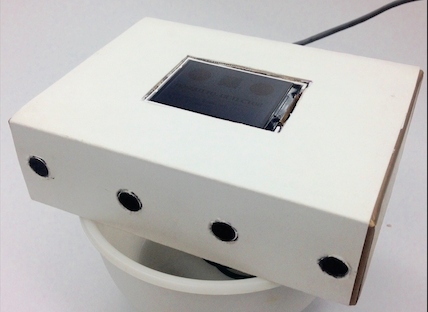
\includegraphics[scale=0.40]{diagView.png}
\newline Figure 1:  Prototype
\end{center}

%------------------------------------------------

\section{Related Research}
Most mosquito related research pertains to large-scale ellimination of mosquitoes to prevent the spread of Malaria. According to the World Health Organization's estimates from December 2015, there were 214 million cases of Malaria and 438,000 Malaria deaths in 2015 \cite{malaria}. To combat this epidemic, the Bill \& Melinda Gates foundation have funded Intellectual Ventures LLC to build a prototype of the ``Photonic Fence'', a large scale mosquito killer. While the Photonic Fence, does use wing beat frequency to identify mosquitoes, it surprisingly does not use any microphones. Instead, the photonic fence consists of lasers and cameras to identify wing frequency using light \cite{photonicFence}. The photonic fence works by using infra-red LED lamps to create a plane of light between two posts. The posts are made of highly reflective material so that light is bounced back towards its source and any insects crossing along the fence will be identified by their shadows. Once an insect is detected, a non-lethal laser tracks the insect to determine its size, wing frequency, and other characteristics which reveal whether the insect is a female mosquito or not. If so, a lethal laser is fired towards the mosquito to literally zap it out of thin air \cite{photonicFenceWiki}. 

Researchers from the Photonic Fence project have claimed that the sound of a mosquito is too faint to detect from a distance over background noise \cite{photonicFence}. However, MIT researchers Fadel Adib and Dina Katabi have developed antenna arrays that can essentially ``see'' through walls by emmitting and detecting Wifi signals across them. This involves highly precise cancellation of background signal so that the very faint reflection of Wifi that has crossed the wall in both directions can be detected over the much higher signal of Wifi that was reflected off the wall instead of crossing it. This is acheived using a smoothed MUSIC algorithm to compute the power received along a particular direction, despite background noise. \cite{wivi}. Inspired by this research, we believe a similar approach could work using a microphone array to detect the highly recognizable sound of a mosquito. 

%------------------------------------------------

\section{Design and Implementation}

\subsection{Overview}

Our device consists of four MAX4466 electret microphones with adjustable gain and a 2.2" LCD TFT display, all connected to the STM32F4 Discovery board. The board collects audio data from the microphones, performs an FFT, then runs the FFT output through a pre-trained neural network. The results of the neural network are then displayed on the screen.

\begin{center}
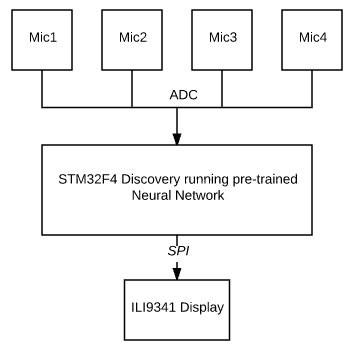
\includegraphics[scale=0.45]{overview.png}
\newline Figure 1: Design Overview
\end{center}

The neural network was trained on a laptop using WEKA, open source machine learning software from the University of Waikato. During development, we transfered audio data from the microphones to the computer over USB, and then trained the neural network with it. We then use the trained neural network to process audio data in real time on the STM32F4. 

\subsection{Microphones and ADC}

We considered several techniques for sampling four microphones simultaneously. One option was to use the internal microphones on 4 different boards and use SPI to communicate meta data from each slave board to a master board. We deemed this to be unecessarily cumbersome. Instead, we purchased 4 external microphones and connected them to 4 ADC pins. We considered sampling each microphone from a separate ADC but instead opted for `scan mode'. Scan mode is an ADC setting that allows developers to assign a sequence of ADC channels to be sampled in quick succession. Figure 3, taken from the STM32F4 Reference Guide, shows an example sequence that uses 7 different ADC channels, some repeated, each with a different sample time.

\begin{center}
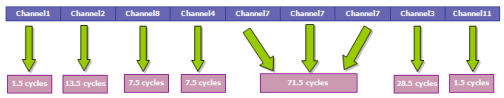
\includegraphics[scale=0.43]{scanMode.png}
\newline Figure 3: ADC Scan Mode
\end{center}

The ADC only has a single register to store the value of the last conversion. There are two ways to read this value: the first is to configure an interrupt to trigger after each channel is sampled, the second is to configure the DMA controller to copy the data of the channels into a defined memory location\cite{ADCTutorial}. In the first method, the ADC sets an EOC flag at the end of every channel's conversion. When this flag is set, an interrupt can read the ADC-DR register to optain the value and reset the EOC flag to signal the ADC to convert another sample. Instead, we opted to use the DMA technique, which is considerably faster. We configured the DMA controller to copy the data of all 4 channels to a designated buffer, all at once, at 
the end of each channel sequence conversion. 

\subsection{Display}

Our display is a 2.2" LCD TFT display with an ILI9341 LCD driver. It has 240 x 320 pixels resolution and 16bit or 18bit color depth. To communicate with the display, we used a graphics library written by Tilen Majerle for the STM website \cite{library}. 
This library used DMA for SPI, and window/page settings were used before sending data to the LCD to reduce time. 

Our display was connected to the board as shown in Figure 4. 
\begin{center}
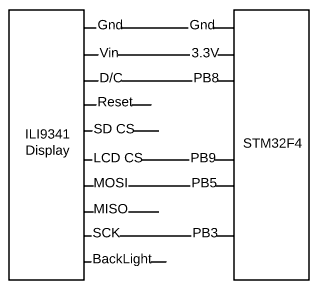
\includegraphics[scale=0.45]{displayPins.png}
\newline Figure 4: Display Pins
\end{center}

We wrote the Display and Microphone code in two separate Git branches. Since they both used the DMA controller we had to separate their functionality onto two separate DMA streams when we merged the branches. The ADC uses DMA2-Stream4 whereas the display used DMA2-Stream0.

DMA-SPI lib: http://stm32f4-discovery.net/2016/04/hal-library-33-dma-extension-for-spi-on-stm32fxxx/
ILI9341 lib: http://stm32f4-discovery.net/2014/04/library-08-ili9341-lcd-on-stm32f429-discovery-board/

\subsection{Data Collection}
Data needed to be obtained from the system in order to create and train a neural network capable of determining the angle and distance of a sound source. This was done using serial USB communication between the board and a computer. When compiled with the 'SERIAL' flag defined, the system will read the serial input waiting for a special character. After receiving this character, the system will take a sample, process the FFT and then transmit the data back over the serial line. A python program was written to collect and save this data.

The training set consisted of 120 samples, 10 samples taken at 3 different angles and 4 different distances along those angles. This data was then assembled by another small python program into a file format usable by WEKA, where the neural net was trained.

\subsection{Signal Processing and Machine Learning}
-- FFT?
-- Neural Network?
-- Interpreting the output of the neural network?
-- Drop data set into weka, choose learning parameters, run algoritm, check error on training set. See file 'DistOUT.txt' and 'AngOUT.txt'

\subsection{Code Structure}
Essentially the hardware is initialized, the main screen is shown and then the main loop is run. The main loop obtains a sample, then calculates its estimate of the distance and angle, then displays the result. Under the data collection mode, the system does the same thing, but waits for serial input to trigger the data collection. Functions were defined to calculate a general neural network output, and the specific coefficients trained by WEKA reside in the 'NN.h' file as global variables.

The most important and most used function is 'obtainSample()' which activates the interrupt timer, beginning data collection. It then takes the gathered samples, performs the FFT and assembles the data into one output array. The functions 'calc\_distance()' and calc\_ang()' then perform the neural network calculations if the macro 'USE\_NN' is defined, or perform a linear regression if the macro 'USE\_LR' is defined. The result is output to the screen using library functions.

%------------------------------------------------

\section{Results and Testing}

Since testing with live mosquitoes would be challenging, we tested our device by playing 600Hz sinewaves from our phones. We moved the phone around the device and confirmed that the screen displayed movement of the audio source. 
%------------------------------------------------

\section{Conclusion}

Future work would be to add lasers. Train the neural net more thoroughly. Interpret the neural net output better. 

\begin{center}
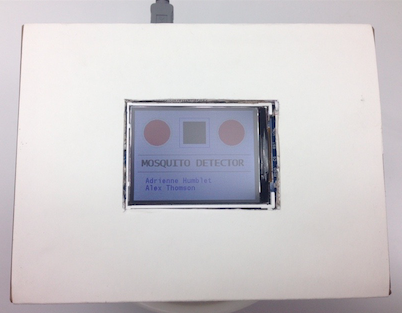
\includegraphics[scale=0.40]{topView.png}
\newline Figure 6:  Top View of Prototype
\end{center}

%----------------------------------------------------------------------------------------
%	REFERENCE LIST
%----------------------------------------------------------------------------------------

\begin{thebibliography}{99} % Bibliography - this is intentionally simple in this template

\bibitem{malaria} http://www.who.int/mediacentre/factsheets/fs094/en/

\bibitem{photonicFence} http://www.intellectualventureslab.com/work/photonic-fence

\bibitem{photonicFenceWiki} https://en.wikipedia.org/wiki/Mosquito-laser

\bibitem{wivi} Fadel Adib and Dina Katabi, See Through Walls with Wi-Fi! https://people.csail.mit.edu/fadel/papers/wivi-paper.pdf 

\bibitem{ADCTutorial} http://survivalengineer.blogspot.com/2013/03/stm32f4-and-most-of-what-you-ever.html

\bibitem{library} http://stm32f4-discovery.net/2014/04/library-08-ili9341-lcd-on-stm32f429-discovery-board/

\bibitem{ADCRefGuide} TMS320x2833x Analog-to-Digital Converter
(ADC) Module Reference Guide. http://www.ti.com/lit/ug/spru812a/spru812a.pdf

\bibitem{libOptimization} Requiem. ILI9341 LCD Driver + STM32F4 + DMA. June 2015. http://www.requiem-projects.com/en/ili9341-lcd-driver-stm32f4-dma/





\end{thebibliography}

%----------------------------------------------------------------------------------------

\end{multicols}

\end{document}
